\section{Módulo Android}

O módulo Android do sistema UMISS tinha como resultado uma aplicação mobile que 
funcionasse nas versões 4.4 e acima do sistema operacional Android. Essa aplicação
seria responsável por avisar os monitores de um paciente caso alguma não esteja de
acordo com o paciente. Para isso foi implementado um sistema de Push Notification
utilizando o serviço Firebase Cloud Message, o \textit{backend} consegue enviar 
notificações para o Android através da biblioteca PyFCM, então a cada sinal identificado
que o \textit{backend} sinalize como anormal, o Android recebe uma notificação.

Também era esperado que a aplicação \textit{mobile} seria capaz de visualizar
os sinais em forma de gráfico. Esse resultado foi alcançado com sucesso utilizando
a biblioteca GraphView, ao usuário monitor realizar \textit{login} na aplicação será
feito uma requisição no servidor e então será criado os gráficos de batimentos cardiáco
e de temperatura.

\begin{figure}[h!]
    \begin{center}
        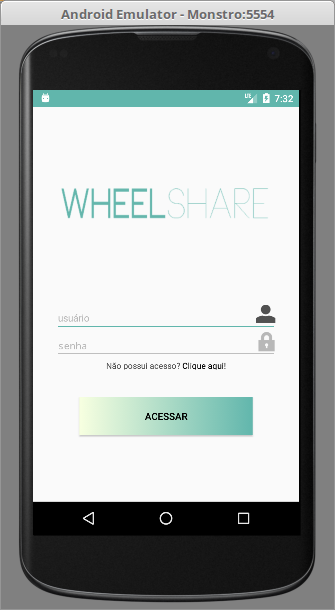
\includegraphics[scale=0.5]{figuras/android2.png}
    \end{center}
    \caption{Página inicial do aplicativo.}
    \label{fig:android2}
\end{figure}

\begin{figure}[h!]
    \begin{center}
        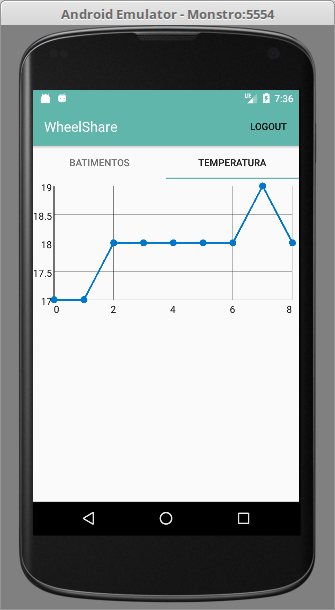
\includegraphics[scale=0.5]{figuras/android1.png}
    \end{center}
    \caption{Visualização dos dados no aplicativo.}
    \label{fig:android1}
\end{figure}





